\documentclass[11pt, oneside]{article} 
\usepackage{geometry}
\geometry{letterpaper} 
\usepackage{graphicx}
	
\usepackage{amssymb}
\usepackage{amsmath}
\usepackage{parskip}
\usepackage{color}
\usepackage{hyperref}

\graphicspath{{/Users/telliott/Github/calculus_book/png/}}
% \begin{center} 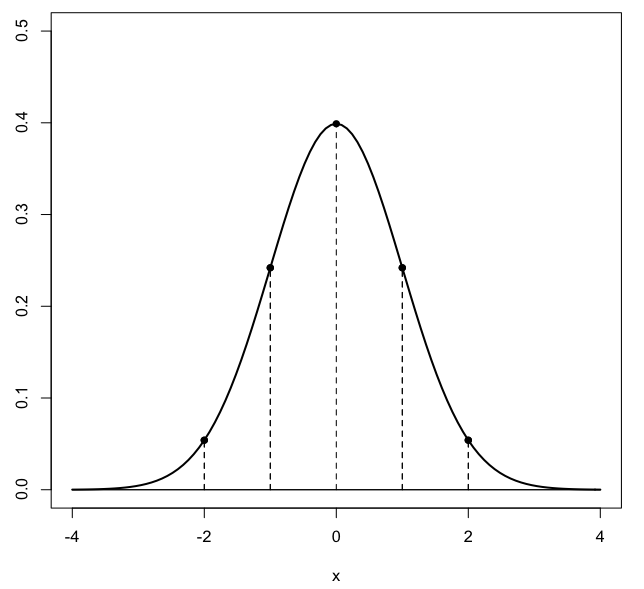
\includegraphics [scale=0.4] {gauss3.png} \end{center}

\title{Slope of a parabola}
\date{}

\begin{document}
\maketitle
\Large

In this chapter,  we show how to find the slope of parabola at any point using classical methods.

\subsection*{part 1}
Consider the simplest parabola:  $y = x^2$.

The point $(1,1)$ is on the curve, because $(x = 1, y = 1)$ satisfies the equation $y = x^2$.

\begin{center} 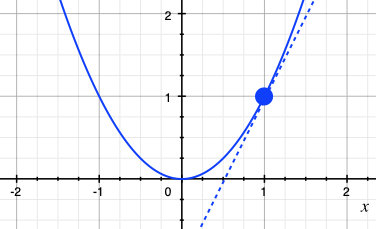
\includegraphics [scale=0.50] {para11.png} \end{center}

Suppose we know that the slope of the tangent to the curve at the point $(1,1)$ is equal to $2$.

(Using calculus to find this result is trivial, we'll also show a non-calculus method in part three, below).  

The equation of the tangent line is
\[ y_2 - y_1 = m(x_2 - x_1) \]
Plugging in for $(x_2, x_1) = (1,1)$ (and just writing $(x,y)$ for $(x_1,y_1)$:
\[ y - 1 = 2(x - 1) \]
\[ y = 2x - 1 \]

Now suppose that we knew only the parabola and this slope, but we did not know the point where the tangent meets the curve, and so do not know the $y$-intercept.

We have the equation of a line:
\[ y = 2x + y_0 \]

We seek points which are simultaneously on the line and the curve.  They must satisfy both equations.

Since this is a tangent line, we seek the value for which this expression has only a single solution.  The tangent "kisses" the curve at a single point.

So, substitute for $y$ from the equation for the curve:
\[ x^2 = 2x + y_0 \]
\[ x^2 - 2x - y_0 = 0 \]

Now look at the quadratic formula we would use to solve this equation for $x$:
\[ x = \frac{-b \pm \sqrt{b^2 - 4ac}}{2a} \]

There is a single solution when the part under the square root (called the discriminant) is equal to zero.

\[ b^2 - 4ac = 0 \]
\[ b^2 = 4ac \]
\[ (-2)^2 = 4(-y_0) \]
\[ y_0 = -1 \]
Therefore, the equation of the tangent line is $y = 2x - 1$, which matches what we had before.

In general, $y = 2x + y_0$ is a \emph{family} of lines.  For $y_0 = -1$, there is a single solution for $x$ to be both on the line and the parabola.  For $y_0 < -1$, there are no solutions, while for $y_0 > -1$ there are two solutions, because the line actually traces out a secant of the parabola, passing through the curve at two points.

\subsection*{part 2}
Now suppose we have the same parabola and a point not on the parabola, but in the plane and outside of the "cup" of the parabola, such as $(3,5)$.  We seek the equations of tangent lines to the parabola that go through this point.  
\begin{center} 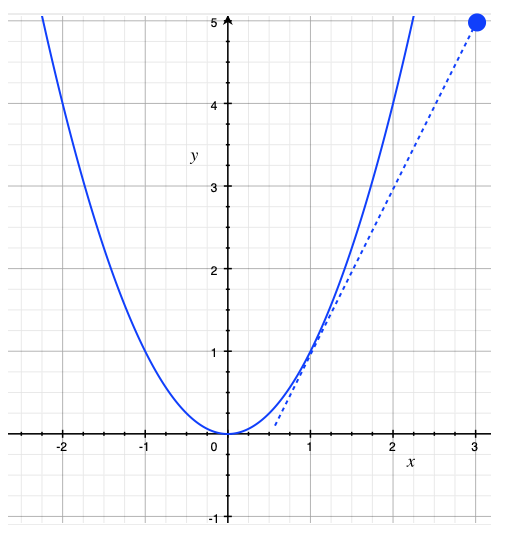
\includegraphics [scale=0.50] {para12.png} \end{center}

There will be two of them.  We show just one in the figure.

The equations of lines passing through this point, with different slopes $m$ are given by:

\[ (y_2 - y_1) = m(x_2 - x_1) \]
Here, let $(x_2,y_2)$ be $(3,5)$ and then multiply by $-1$, and drop the subscript, to obtain:

\[ y - 5 = m(x - 3) \]

Since values of $(x,y)$ are both on the line and the parabola $y=x^2$, we can plug in for $y$:
\[ x^2 - 5 = mx - 3m \]
\[ x^2 - mx + (3m - 5) = 0 \]

As before, solutions are given by the quadratic equation.  The value of the slope $m$ giving a single solution (zero discriminant) is:
\[ (-m)^2 - 4(3m - 5) = 0 \]
\[ m^2 - 12m + 20 = 0 \]
\[ (m - 2)(m - 10) = 0 \]
\[ m = 2, \ \ \ m = 10 \]

We knew the first one already, because the point $(3,5)$ is on the line $y = 2x - 1$.  This is the tangent to the curve at $(1,1)$, which has slope $m = 2$.
\begin{center} 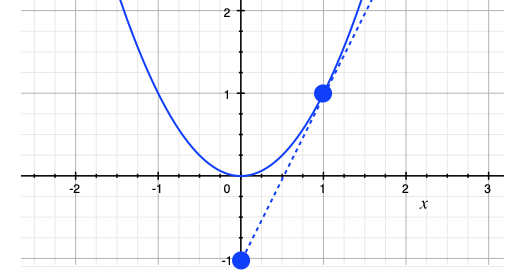
\includegraphics [scale=0.50] {para13.png} \end{center}

Actually, there is always another solution.  Any vertical line (with infinite slope) passes through only a single point on the parabola.

Basically what this amounts to is that in the equation
\[ x = \frac{m \pm \sqrt{(-m)^2 - 4(3m - 5)}}{2} \]

as $m$ gets very large, only the term $(-m)^2$ matters under the square root, so we have
\[ x = \frac{m \pm \sqrt{(-m)^2}}{2} \]
if we choose the negative root, then as $m \rightarrow \infty$, $m - \sqrt{m^2} \rightarrow 0$.

\subsection*{part 3}
Now suppose we are given the same parabola again and also a point on it such as $(x_1,y_1)$.  

Any line through that point has the equation:
\[ y - y_1 = m(x - x_1) \]

To find the equation of a tangent line through that point we need the slope $m$.

If there is a point $(x,y)$ that is on the line and \emph{also} on the parabola, it must satisfy $y = ax^2$ as well, so:
\[ ax^2 - ax_1^2 = m(x - x_1) \]
\[ ax^2 - mx - ax_1^2 + mx_1 = 0 \]

Certainly $x = x_1$ is a solution.

The value of $m$ must be such that there are \emph{no other solutions}.

Write the quadratic equation to solve for $x$:
\[ x = \frac{m \pm \sqrt{m^2 - 4a(mx_1 - ax_1^2)}}{2a} \]

There is a single solution when the discriminant is zero, that is, when
\[ x = \frac{m}{2a} \]
\[ m = 2ax \]

Since $x = x_1$ for the tangent line
\[ m = 2ax_1 \]
as expected.

The slope of the tangent line is $2ax_1$ and in particular, at the point $(1,1)$, the slope is equal to $2$.

That's the answer, but there are two points to follow up on.  We should plug the answer into these two equations and check what happens.  We need
\[ ax^2 - mx - ax_1^2 + mx_1 = 0 \]
and
\[ m^2 - 4(mx_1 - ax_1^2) = 0 \]

For the first one:
\[ ax^2 - 2ax^2 - ax_1^2 + 2ax_1 \]
This is certainly equal to zero when $x = x_1$.

Then
\[ m^2 - 4a(mx_1 - ax_1^2) \]
\[ 4a^2x^2 - 4a(2ax_1 - ax_1^2)  \]
\[ 4a^2x^2 - 8a^2x_1^2 + 4a^2 x_1^2 \]
is also equal to zero when $x = x_1$.

\subsection*{alternate solution}
\begin{center} 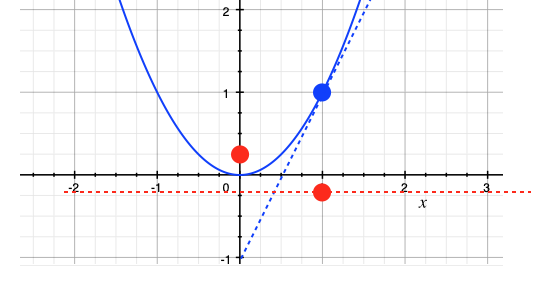
\includegraphics [scale=0.50] {para14.png} \end{center}

A parabola is defined geometrically by its focus, which is the point $(p,0)$ for a centered parabola.

The focus is paired with a directrix, which is the line $y = -p$ for a vertex at the origin.  

All points on the parabola lie at the same distance $d$ from the focus and the directrix.

A relatively advanced fact about the parabola is that any tangent line intersects the $y$-axis at the same distance $d$ from the focus.

\begin{center} 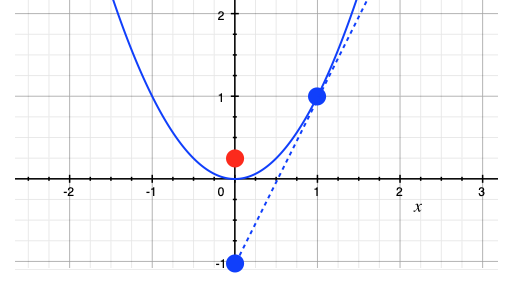
\includegraphics [scale=0.50] {para15.png} \end{center}

Which is to say that if we draw a triangle in the above diagram using the two blue points and one red one, the two blue points are the vertices of equal angles and the triangle formed is isosceles.

For $y = x^2$, consider the point $(x,x^2)$, and find the distance to the focus squared as 
\[ d^2 = (x)^2 + (x^2 - p)^2 \]
\[ d^2 = x^2 + x^4 - 2x^2p + p^2 \]

Call the $y$-intercept $k$ so then 
\[ k + d = p \]
\[ d^2 = p^2 - 2pk + k^2 \]

Equating the two expressions:
\[ p^2 - 2pk + k^2 = x^2 + x^4 - 2x^2p + p^2 \]
\[ k^2 - 2pk = x^2(1 + x^2 - 2p)  \]

In this case, we know $x = 1$ and $p = 1/4$ so
\[ k^2 - \frac{k}{2} - (2 - \frac{1}{2}) = 0 \]

We factor to obtain:
\[ (k + 1)(k - \frac{3}{2}) = 0 \]

$k = -1$ was our solution above.

I am a little uncertain as to the significance of the other solution ($ k = 3/2$).  But it cannot be an accident that this is the $y$-intercept of the line perpendicular to the tangent that goes through the point of tangency.

\subsection*{further comment}

The slope of the parabola has some simple interesting properties.  For example, pick any two points $(x,y)$ and $(x',y')$ on our standard parabola.

The slope of the line that connects those two points is equal to the slope of the parabola at the point whose $x$-value is halfway in between.  
\begin{center} 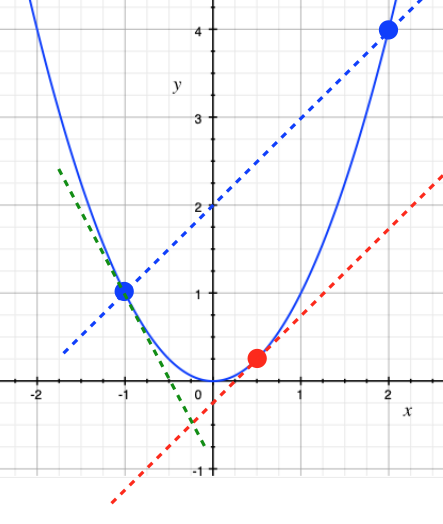
\includegraphics [scale=0.50] {para19.png} \end{center}

For the first part:
\[ m = \frac{y'-y}{x'-x} \]
\[ = \frac{ax'^2 - ax^2}{x'-x} \]
\[ = a \ [ \ \frac{x'^2 - x^2}{x' - x} \ ] \]
\[ = a(x' + x) \]

For the midpoint
\[ x_m = \frac{1}{2} (x' + x) \]
and the slope is
\[ 2a \cdot \frac{1}{2} (x' + x) \]
\[ = a(x' + x) \]

A similar result is that if we pick any two points $(x,y)$ and $(x',y')$, and draw their slopes, the point where the two slope lines meet has its $x$-value exactly halfway in between $x$ and $x'$.

\subsection*{circle}

Suppose we have a unit circle and an external point $(x,y)$.  We wish to find the equation of the tangent line to a point on the circle.  Call that point $(a,b)$.

Circles are special.  Any tangent is perpendicular to the radius at the point of tangency.  

The line through $(a,b)$ and the origin has slope $b/a$ since
\[ m = \frac{b - 0}{a - 0} \]

If we have two lines with slopes $m_1$ and $m_2$ and they are perpendicular, the product is $-1$.  So the tangent to the circle at $(a,b)$ has slope $-a/b$ and the line through $(x,y)$ and $(a,b)$ is

\[ -\frac{a}{b} = \frac{y - b}{x - a} \]
\[ - ax + a^2 = by - b^2 \]

We also have that $a^2 + b^2 = 1$ so
\[ ax + by = 1 \]

Substitute into the equation of the circle:
\[ a^2 + (\frac{1 - ax}{y})^2 = 1 \]
\[ a^2y + 1 - 2ax + a^2x^2 = y \]
\[ (y + x^2)a^2 - 2xa + (1 - y) = 0 \]

We have a quadratic in $a$.  For a particular $x$ and $y$, we can solve for $a$.

\subsection*{ellipse}
I found a problem on the web that extends this to the ellipse:

\url{https://math.stackexchange.com/questions/834392/equations-of-lines-tangent-to-an-ellipse}

In working that problem, I ended up with a quartic equation (fourth power).  This is, quite literally, a mess.

Here's a great idea for ellipse problems:  Stretch and rescale the problem to one involving a circle, by using a \emph{change of variable}.  Suppose the ellipse is
\[ \frac{x^2}{a^2} + \frac{y^2}{b^2} = 1 \]
Let $x = au$ and $y = bv$.  Then
\[ \frac{a^2u^2}{a^2} + \frac{b^2 v^2}{b^2} = 1 \]
\[ u^2 + v^2 = 1 \]

The ellipse has become a unit circle!

Apply the same transformation to any points in the problem, solve the problem, and then reverse the transformation.

\end{document}